\documentclass[conference]{IEEEtran}
\usepackage{blindtext, graphicx}


% *** CITATION PACKAGES ***
%
%\usepackage{cite}
% cite.sty was written by Donald Arseneau
% V1.6 and later of IEEEtran pre-defines the format of the cite.sty package
% \cite{} output to follow that of IEEE. Loading the cite package will
% result in citation numbers being automatically sorted and properly
% "compressed/ranged". e.g., [1], [9], [2], [7], [5], [6] without using
% cite.sty will become [1], [2], [5]--[7], [9] using cite.sty. cite.sty's
% \cite will automatically add leading space, if needed. Use cite.sty's
% noadjust option (cite.sty V3.8 and later) if you want to turn this off.
% cite.sty is already installed on most LaTeX systems. Be sure and use
% version 4.0 (2003-05-27) and later if using hyperref.sty. cite.sty does
% not currently provide for hyperlinked citations.
% The latest version can be obtained at:
% http://www.ctan.org/tex-archive/macros/latex/contrib/cite/
% The documentation is contained in the cite.sty file itself.

% correct bad hyphenation here
\hyphenation{op-tical net-works semi-conduc-tor}


\begin{document}
%
% paper title
% can use linebreaks \\ within to get better formatting as desired
\title{Proposal for Team Building Application}


% author names and affiliations
% use a multiple column layout for up to three different
% affiliations
% \author{\IEEEauthorblockN{Michael Goff}
% \IEEEauthorblockA{Department of Computer Science\\
% North Carolina State University\\
% Raleigh, North Carolina 27606\\
% Email: magoff2@ncsu.edu}
% \and
% \IEEEauthorblockN{Shashank Jha}
% \IEEEauthorblockA{Department of Computer Science\\
% North Carolina State University\\
% Raleigh, North Carolina 27606\\
% Email: sjha5@ncsu.edu}
% \and
% \IEEEauthorblockN{Jingjuan Deng}
% \IEEEauthorblockA{Department of Computer Science\\
% North Carolina State University\\
% Raleigh, North Carolina 27606\\
% Email:jdeng8@ncsu.edu}
% \and
% \IEEEauthorblockN{Bhaskar Sinha}
% \IEEEauthorblockA{Department of Computer Science\\
% North Carolina State University\\
% Raleigh, North Carolina 27606\\
% Email:bsinha@ncsu.edu}}


% for over three affiliations, or if they all won't fit within the width
% of the page, use this alternative format:
% 
\author{\IEEEauthorblockN{Michael Goff\IEEEauthorrefmark{1},
Shashank Jha\IEEEauthorrefmark{2},
Jingjuan Deng\IEEEauthorrefmark{3} and
Bhaskar Sinha\IEEEauthorrefmark{4}}
\IEEEauthorblockA{Department of Computer Science, North Carolina State University, \\
Raleigh, North Carolina 27606\\ 
Email: \IEEEauthorrefmark{1}magoff2@ncsu.edu \\
\IEEEauthorrefmark{2}sjha5@ncsu.edu \\
\IEEEauthorrefmark{3}jdeng8@ncsu.edu \\
\IEEEauthorrefmark{4}bsinha@ncsu.edu}}


% make the title area
\maketitle


\begin{abstract}
A study was performed to investigate the need for a team formation application based on the previous experiences of surveyed students in
various team environments. The results of the study indicated that students generally had a decent time in their previous team experiences
but there were some common minor complaints around topics like communication and sharing the workload. Students also much preferred creating
their own teams, rather than having one assigned on their behalf. 

After considering user preferences we are proposing an intelligent team 
formation application using one of three different approaches. The first approach would allow users to create a group and allow other users to 
apply based on posted skill sets that were requested from the team lead. The second approach would create a pool of users, typically from a class 
roster, and intelligently match up groups based on their skill sets parsed from a third party service like LinkedIn. The final proposed solution
is a system where users can provide a list of their preferred projects and then will be intelligently sorted into groups using a weighted lottery
with other skill set considerations. 

After developing these approaches, they will be tested on potential users to determine which one would be the best overall solution to forming 
a team in a classroom environment. 

\end{abstract}


% Note that keywords are not normally used for peerreview papers.
\begin{IEEEkeywords}
Teams, software, matching, proposal.
\end{IEEEkeywords}






% For peer review papers, you can put extra information on the cover
% page as needed:
% \ifCLASSOPTIONpeerreview
% \begin{center} \bfseries EDICS Category: 3-BBND \end{center}
% \fi
%
% For peerreview papers, this IEEEtran command inserts a page break and
% creates the second title. It will be ignored for other modes.
\IEEEpeerreviewmaketitle



\section{Introduction}
One of the most frequent classroom interactions is team formation. Projects in classes often require the formation of a team to complete a larger task.
Professors will often let students work amongst themselves to figure out an ideal team, but sometimes they want to simulate a work environment and assign
teams randomly. Sometimes teams formed in these two ways lead to problems in productivity and disputes may occur. 

A solution to these problems in teams may be to create an application to intelligently let students create teams or have teams created for them. However,
a collection of background information was required to see the feasibility of such an application. With background data in mind, we have come up with three
approaches to the team formation problem. The first approach would be to allow users to create a group with specific needs and let other students apply.
The second approach would be to intelligently match students together from a pool based on their areas of expertise. The third solution would be to 
have users supply a list of preferred project topics and then the application would sort these users into groups in a weighted lottery while considering
areas of expertise and compatibility.

\section{Literature Review}
Matching is widely used in social websites to find friends and recommend news. Developers have designed an approach to recommend news stories on Twitter to users, based on their preferences \cite{twitter}. A paper on Social Matching System claims that the difficulties in matching are the set of key research challenges, and the roster of appropriate methods are all ill-defined. The method to solve these is focusing on things people most care about in different situations. In our design, we should focus on the quality that people most care about to get better matching result.

We can also implement team formation by allocating human resources to a team. People used search-based technique such as genetic algorithm and Tabu search to optimize random allocation in project resources management \cite{searchbased}. There has been a dramatic increase in work on Search Based Software Engineering. This technique applies meta-heuristic search techniques such as genetic algorithms, simulated annealing and tabu search to software engineering problems. 

According to previous research, we will consider optimizing our design in some ways such as ranking results in an appropriate order, tuning criteria to ensure an available result and adding limitations in a randomized algorithm.

\section{Study}
In order to figure out how to approach a team building application we needed
to determine what the user needs. We concluded that the
application could be used from both a teacher's perspective and a student's 
perspective; however, we decided to focus our study on the student aspect since
they are the users who are most affected from a team assignment.

\subsection{Research Questions}
In this section we describe the different questions we put forth in a Google Survey 
and why we decided to ask each question. We ultimately decided on a Google Survey in
order to get a quick response from a larger pool of people. With an online survey it
is easy to push it out to many peers including those beyond the scope of the class.

\textbf{Q1: Are you a master's student?}

We wanted to ask this question to get a sense of the type of students who were responding
to our survey. Master's students are different from undergraduate students because they
have different workloads and, as a result, different experiences in team projects.

\textbf{Q2: How many different team projects do you work on in a year?}

We wanted to get a sense of how often people work in group projects. The more group 
projects they participate in, the more chances they would have of a group being
especially poor or exceptional. It would provide a better perspective on the
individuals experience overall.

\textbf{Q3: Do you face problems finding team members with specific skill sets?}

This relates to our idea for some of the application approaches. We want to find a way
to automate the process of finding a variety of skills and forming teams with the widest
breadth of expertise possible. When you have different people who are experts in different areas
it may be easier to distribute the workload among the team.

\textbf{Q4: Which services have you used to form teams before?}

We wanted to ask this question to see what kinds of tools students already use to form teams. 
By having the perspective of the current tools students use, we can investigate what makes those 
tools useful and what kind of drawbacks they have. 

\textbf{Q5: What experiences did you have with those team members which you found?}

We asked this as an open ended question because we wanted to see what kinds of different
experiences the users have previously had. Our team has an idea of what could go wrong on
a group project but we wanted to avoid anchoring the survey participants to a specific 
problem and see if there were other pieces that we were missing. 

\textbf{Q6: On a scale of 1 to 5, five being the highest, how successful were your
previous team projects?}

This question was meant to gauge the success students have had in previous projects. If the 
responses were mostly negative, we could use it to justify a need for a new tool in team formation.

\textbf{Q7: What were some problems that you had with team members in the past?}

We wanted to dig into those negative experiences users had about working others to see if there
were some potential problems that we could help address in our application. This was another open
ended question where we wanted to explore the types of issues that could occur without framing the 
participant's thoughts. 

\textbf{Q8: What other qualities aside from technical expertise do you look for in a potential team member?}

We know the main benefit of finding a good team member is their technical expertise, but we wanted
to dig deeper and see if there were other major aspects that were worth exploring like social 
benefits or other unknown intangibles. 

\textbf{Q9: In general, while doing a project, which is better for you? Randomly Assigned Teams or
Freely Formed Teams.}

This was a two option question. We wanted to know what students would prefer in a team project. 
If there was an overwhelming preference for one or another, we could shape our application to use 
student input in forming teams instead of an emphasis on matching using algorithms. 

\textbf{Q10: While doing a project do you prefer to collaborate online or in person with your team?}

This was another social test of sorts. We wanted to judge whether an online application would be 
beneficial for these users. If they prefer to work online then perhaps the social aspects of a team
would not be as important since there would be much less face-to-face social interaction. 

\textbf{Q11: How often do you assess a potential team member's skills before forming a team?}

We wanted to see how much a user has even thought about or considered the skills of other students
before committing to working with them in a team. If students thought a lot about those considerations
then the usefulness of an application for matching based on skills would be beneficial. 

\textbf{Q12: If there was a potential web application for team creation, would it be helpful to you?}

This was a direct question relating to our application. We wanted to gauge how much interest there 
would be in an application that could help students to form teams. If there was a lot of interest
we could be really making a difference in the ease of team formations with our application. 

\section{Survey Results}
We received 41 responses in our survey at the time of writing through the Google Survey. Below
is a collection of the results and our thoughts regarding the outcome. 

\subsection{Results}

\begin{figure}[!ht]
\centering
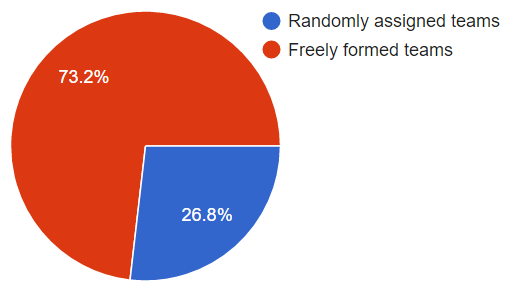
\includegraphics[width=2.5in]{free_assigned}
\caption{Randomly Assigned vs. Freely Formed Teams}
\label{random_free}
\end{figure}

In figure \ref{random_free}, most of the participants much preferred to freely form teams over random
assignment. This result indicates that students would rather control their own group by having a say
on who is involved. When it is a randomly assigned team there is always a risk of having a known
slacker in the group who would have been explicitly avoided if it were a student chosen team. Another
reason could be that students would prefer to work with their friends on a project since they already
know the kind of work ethic their peers have and enjoy their existing time together. 

\begin{figure}[!ht]
\centering
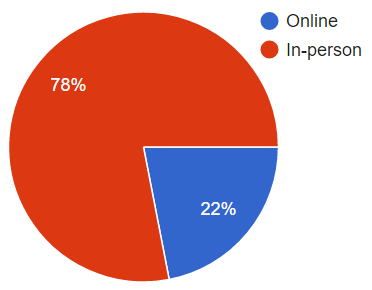
\includegraphics[width=2.5in]{online_person}
\caption{Would you rather work together online or in person?}
\label{online_person}
\end{figure}

Similar to freely formed teams, working in person was much more popular than working online by a very similar
ratio, as seen in figure \ref{online_person}. The preference seems to imply that groups are
more successful that work together in person rather than online. The question format could have been more specific
about online meeting to include web video conferences or something similar. Perhaps ideas and best spread in person
rather than through the Internet. The results also imply that a heavier social similarity will lead to a stronger
likelihood of success among teams.

\begin{figure}[!ht]
\centering
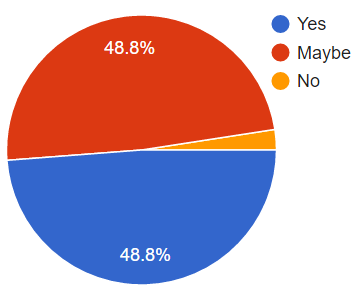
\includegraphics[width=2.5in]{useful}
\caption{Would a potential web application be useful to you?}
\label{useful}
\end{figure}

The results from Q12 were promising for our application. As shown in figure \ref{useful}, most of the
participants marked either yes or maybe in considering the utility of a team-building application.
In retrospect, it might have been better to make this kind of a question a yes or no style of question.
The addition of maybe as an answer choice lets the survey participant answer without actually considering
the application itself. However, about half of the participants did explicitly mark 'yes' for the question
so some interest could exist. 

\begin{figure}[!ht]
\centering
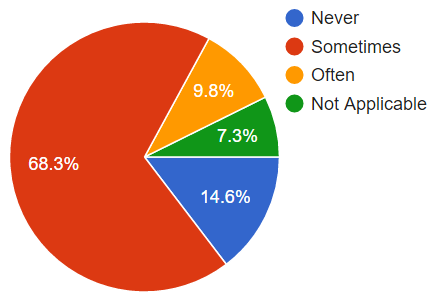
\includegraphics[width=2.5in]{problems_finding_members}
\caption{Have you ever had problems finding team members with specific skill sets?}
\label{finding_members}
\end{figure}

Question 3 did not present much surprise in its results, shown in figure \ref{finding_members}. The choice 'Sometimes'
took a vast majority of the votes as students seem to have a problem from time to time. This is another instance
of a question where 'sometimes' probably should not have been an option or this question should have been presented
as a scale. We are unable to get much real information from these results. There was a small edge of people never
having problems over those who have problems all the time though, but that might just be a result of the somewhat
small sample size. 

\begin{figure}[!ht]
\centering
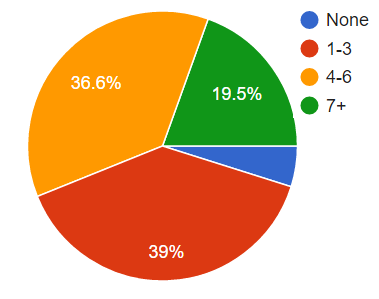
\includegraphics[width=2.5in]{num_team_projects}
\caption{What's the number of team projects you have worked on in a year?}
\label{num_team_projects}
\end{figure}

The spread of the number of team projects that students partake in a year were not too surprising, as seen in figure
\ref{num_team_projects}. About a third participated in 4-6 projects a year which roughly lines up with a full workload
for two semesters of work at school as a graduate student. Having about 40 percent working in only 1-3 projects was somewhat surprising since
that accounts for only about 1-2 projects a semester. Most classes seem to focus on group work, at least here at NC State. 
Perhaps there was some influences of the 25 percent of people who were not master's students taking this survey.

Question 5 was an open end question regarding experiences with team members. Since we avoided asking for any positive or negative experience, we were surprised to see that most of them replied with negative ones. Lack of coordination, work division, different goals, different expectations, schedule conflict, etc were mostly mentioned. In question 7, where we specifically asked for problems they faced in past, responses were similar. Hence, proving our point that existing team creation methods are not perfect. If we can address these problems, our product is sure to have a user base.


Question 8 was again an open ended question. By asking this, we wanted to know what exactly people are looking for beside the technical skills. It would be useful for us to understand our target group. Thus we will design our application and search criteria accordingly.  

\begin{figure}[!ht]
\centering
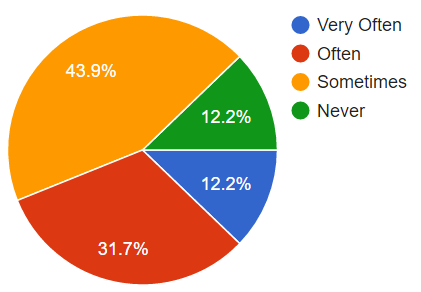
\includegraphics[width=2.5in]{assess_skill}
\caption{How often do you assess the skills of potential team members?}
\label{assess_skill}
\end{figure}

Once again in question 11, we made a mistake by putting in sometimes as an answer choice. As shown in figure
\ref{assess_skill}, 'sometimes' was a dominant answer with about 44 percent of the votes. A better scale would
have been to use a number system to try to split out the 'sometimes' votes into something more granular. These results
otherwise seem to indicate that assessing others skills is a pretty common occurrence with about 44 percent of the votes
spread between 'very often' and 'often' which implies that relevant skills are important to team success. 

\begin{figure}[!ht]
\centering
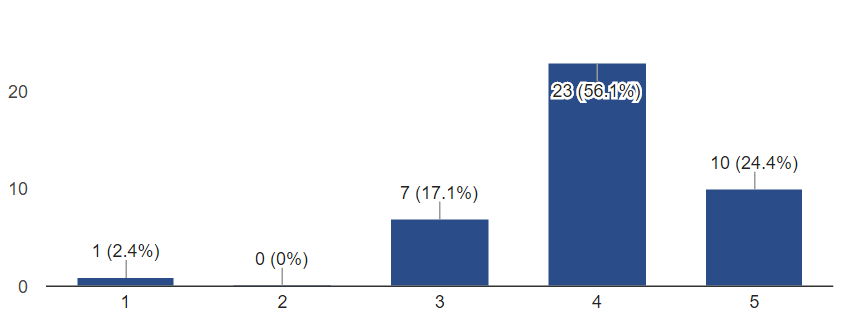
\includegraphics[width=2.5in]{prev_project_success}
\caption{How successful were your previous team projects?}
\label{prev_project_success}
\end{figure}

The success of previous team projects for most survey participants were a 4 out of 5 indicated on figure
\ref{prev_project_success}. The majority of responses were leaning towards more success with the vast majority in the 
4 and 5 categories with a few average experiences at 3. There was only 1 of the 41 participants who had a strongly 
negative experience. We think these statistics can be improved even further with the help of a team generation tool. 
With the tools help, more people can have a better group experience and push the graph more to the right. 
 

\section{Approaches}
First, to start using our application, a user needs to create their profile. Rather than adding all the details one by one, we will be fetching information from their LinkedIn profile. Hence, skill sets, experience, previous project work, etc will all be added in one click. They will also have the option to add (or remove) any more details.

\textbf{Approach 1}

According to our survey, around 78\% of people face a problem finding team members with specific skill sets. Hence, we want to address that problem. The first approach is based on what we are already familiar with: a user searching for other team mates. But rather than showing other users randomly, we will display the result according to the number of skill set matches. If a user is looking for team mates who are good in python, database management and web designing, he can add those in search criteria. Then, output will be displayed in descending order of matches. The user can then connect with whoever they are interested in working with. There is also a threshold value that indicates the least percentage of skills that should match. a user will be able to toggle that value depending upon their needs.  

Notice that here user does not only mean a single person. It can also be a team who is looking to add someone with specific skill set. Hence, it can be used to start a team from scratch or help complete one.



\textbf{Approach 2}

Our second approach is targeted for someone under whom a pool of people is already available. The best example can be a professor. Let’s say they have a project in mind for which they want their class to work. One way to divide class into teams would be to let the students decide their team mates by themselves. But doing so would mean they would not be prepared for a real life scenario where they may have to work with new team in office. Thus, there is need of a second approach, which is randomly assigning a team. This poses one big problem. What if all the members have similar skill sets and it does not cover all the requirements for completion of project? It would be much better if the skill sets are distributed in an even way. This way, everyone in the team can take lead in whatever their strong point is. Everyone can contribute to the project. Also, if they are not familiar with other skill sets, they can learn from their own team mates. Hence, it would be a win-win situation.

To achieve optimized random teams, the person in charge needs to define the total number of members in each team and the total number of resources available. Our application will take care of team creation in a fair way. If the user base is only 4-5, the solution provided by us might be not be standing out. But considering the fact that few classes have student count around 100, manually dividing fairly would be exhausting. This is when our second approach comes into play.

\textbf{Approach 3}

The third approach is based on randomly generating algorithm to create project teams. Since we notice that even though 73.2\% percent of participants' experience are freely formed teams, there are still 26.8\% other cases in which people formed teams by randomly assigning. Additionally, in some cases freely formed teams is not practical nor well estimated. So randomly assigned team is a candidate solution to solve these problems. 

Random algorithms are usually used in program testing
\cite{randomtest} and system scheduling\cite{lottery}. This kind of algorithms have some advantages:
(1) Efficiency: since the result is generated by random factors, it saves many time from considering and calculating complex factors.
(2) Fairness: ensure every eligible candidates have the same chance to compete for joining a team. And two separate runs may have different results.
(3) Objectiveness: the result is determined by criteria in  program, not by any person.

 We combine random algorithm and requirement limitations to generate quality teams in a easy way. To illustrate this in an example, assuming we have a talent pool and some topics available(topics are came up by a manager, a faculty, a student or people who wants to form a team). People in the talent pool can choose at most 5  topics which have slots fit for their skills. The topics they choose have different weights according to their preference. There may be several candidates that apply for the same team. In this case, we should have several runs, people who haven't been chosen in the first run will apply for their second topic in the next run. So on and so forth until every candidates find their teams.


\section{Conclusion}

Our study shows the problems in team formation and teammate matching. The survey indicates that most of the participants have problem in finding team members with specific skills. So we will design team formation solutions that focus on searching and matching teammates with skills required. 

Some software solves similar problems such as friends matching, news recommendations and project resource allocation. Inspired by previous research, we designed 3 solutions to solve team formation problem. The first solution is user searches for other team mates by some criteria. The second solution is randomly generating teams in a talent pool. This solution is efficient but the result may not satisfy every team member. The third solution is generating teams using users' preferred list, this solution is a two-way selection.

To evaluate the teams generated in our solution, We collect LinkedIn profiles from the survey as talent pool. It is difficult to make sure every teams are formed perfectly, evaluation should be various according to different situation:
(1) For one individual, evaluate the ability to find optimal team.
(2) For one specific team, evaluate the ability to find optimal team members in talent pool.
(3) For every teams, evaluate the throughput of satisfied scores.








% trigger a \newpage just before the given reference
% number - used to balance the columns on the last page
% adjust value as needed - may need to be readjusted if
% the document is modified later
%\IEEEtriggeratref{8}
% The "triggered" command can be changed if desired:
%\IEEEtriggercmd{\enlargethispage{-5in}}

% references section

% can use a bibliography generated by BibTeX as a .bbl file
% BibTeX documentation can be easily obtained at:
% http://www.ctan.org/tex-archive/biblio/bibtex/contrib/doc/
% The IEEEtran BibTeX style support page is at:
% http://www.michaelshell.org/tex/ieeetran/bibtex/
%\bibliographystyle{IEEEtran}
% argument is your BibTeX string definitions and bibliography database(s)
%\bibliography{IEEEabrv,../bib/paper}
%
% <OR> manually copy in the resultant .bbl file
% set second argument of \begin to the number of references
% (used to reserve space for the reference number labels box)
\begin{thebibliography}{1}
\bibliographystyle{IEEEbib}

\bibitem{matching}
Loren Terveen. Social Matching: A Framework and Research Agenda.  \emph{ACM Transactions on Computer-Human Interaction (TOCHI)}, 2005.\\


\bibitem{twitter}
Owen Phelan. Using twitter to recommend real-time topical news.  \emph{RecSys '09 Proceedings of the third ACM conference on Recommender systems}, 2009.\\

\bibitem{searchbased}
Massimiliano Di Penta. The use of Search-Based Optimization Techniques to Schedule and Staff Software Projects: an Approach and an Empirical Study.  \emph{SOFTWARE—PRACTICE AND EXPERIENCE}, 2009.\\

\bibitem{IEEEhowto:kopka}
H.~Kopka and P.~W. Daly, \emph{A Guide to \LaTeX}, 3rd~ed.\hskip 1em plus
  0.5em minus 0.4em\relax Harlow, England: Addison-Wesley, 1999.
 \\ 

\bibitem{randomtest}
Andrea Arcuri. A Hitchhiker’s Guide to Statistical Tests for Assessing Randomized Algorithms in Software Engineering.  \emph{Software Testing, Verification and Reliability}, 2016.\\

\bibitem{lottery}
Carl A. Waldspurger. Lottery Scheduling: Flexible Proportional-Share Resource Management.  \emph{OSDI 94 Proceedings of the 1st USENIX conference on Operating Systems Design and Implementation}, 1994.\\


\end{thebibliography}

\newpage

\section{Chit words}
\begin{itemize}
    \item bkggaeau
    \item chfxoaua
    \item cjhgooee
    \item ckfhiieo
    \item clfnuuui
    \item dbhfoaui
    \item dcgnauou
    \item ddfdaiia
    \item dhcneieu
    \item dmgneuio
    \item fbdfuuuo
    \item fcgcaeii
    \item flcsaiuo
    \item fmhzoaio
    \item gbljuuue
    \item gccmioio
\end{itemize}

%\vfill

% Can be used to pull up biographies so that the bottom of the last one
% is flush with the other column.
%\enlargethispage{-5in}




% that's all folks
\end{document}


